\chapter{Environment Evaluation} \label{enveva} 
%Para poder evaluar el desempeño del ambiente tendremos que separar los resultados obtenidos entre los 3 experimentos ya que cada uno de ellos media diferentes cosas o diferentes situaciones. Para el primer experimento nos enfocamos en la aceptacion del ambiente entre los primeros usuarios que pudieron utilizar el ambiente como recordaremos los usuarios de ese experimento tomando los resultados de la encuesta, en el segundo experimento se esperaba evaluar el analisis de el nivel de atencion de los usuarios con el sensor kinect en la seccion del experimento 2 discutiremos el porque no se utilizaron estos datos lo que nos dejo con encuestas para evaluar a los usuarios. Por ultimo en el tercer experimentos utilizamos encuesta para evaluar aceptacion y preferencias del usuario, determinar su nivel de atencion manualmente atraves de un video y determinar su nivel de atencion automaticamente con el sensor kinect.
In order to evaluate the performance of the environment we will have to separate the results obtained between the 3 experiments since each of them means different things or different situations. For the first experiment we focused on the acceptance of the environment among the first users who could use the environment as we will remember the users of that experiment taking the results of the survey, in the second experiment was expected to evaluate the analysis of the level of attention of the users with the kinect sensor in the section of experiment 2 will discuss why these data were not used, leaving us with surveys to evaluate users. Finally in the third experiment we used a survey to evaluate user acceptance and preferences, determine their level of attention manually through a video and determine their level of attention automatically with the kinect sensor.

\section{Results experiment 1}
%Cuando los usuarios terminaron de utilizar el ambiente se les realizo una pequeña encuesta, esta encuesta consistía en 5 preguntas sobre su experiencia al utilizar el ambiente preguntas como si se le dificulto utilizarlo o si fue de su agrado los re-cursos mostrados, con el objetivo de obtener retroalimentación de los usuarios para hacer futuras mejoras y modificaciones. La evaluacion del primer prototipo que recordamos fue una actividad de aprendizaje del himno nacional mexicano con la participacion de 10 usuarios, los 10 usuarios concluyeron la actividad hasta el final y contestaron la encuesta que se presento en la tabla \ref{tab:users1}.
When users finished using the environment they were given a small survey, this survey consisted of 5 questions about their experience using the environment questions as if they were difficult to use or if they liked the resources shown, in order to obtain Feedback from users to make future improvements and modifications. The evaluation of the first prototype that we remembered was a learning activity of the Mexican national anthem with the participation of 10 users, the 10 users concluded the activity to the end and answered the survey that was presented in the table \ref{tab:users1}.
\begin{table}
\centering
\small
\captionsetup{font=footnotesize}
\caption{Survey part 1.}
\label{tab:survey1} 

\small
\begin{tabular}{p{7cm} p{3cm} }
\hline{\smallskip}
Question	& Mean\\
\noalign{\smallskip}\hline\noalign{\smallskip}
\small{	From 1-10 how easy it was use the environment? 	}& \small{	9	}\\
\small{	From 1-10, how was your satisfaction about the information displayed in the environment?  	}& \small{	9	}\\
\hline
\end{tabular}
\end{table}

\begin{table}
\centering
\small
\captionsetup{font=footnotesize}
\caption{Survey part 2.}
\label{tab:survey2} 

\small
\begin{tabular}{p{7cm} p{3cm} p{3cm} }
\hline{\smallskip}
Questions & Answer	& Frequency\\
\noalign{\smallskip}\hline\noalign{\smallskip}
\small{	Did you like the idea of using various visual elements? 	}& \small{	Yes	}& \small{	8	}\\
\small{		}& \small{	No	}& \small{	2	}\\\hline
\small{	Was necessary technical assistance to use the environment? 	}& \small{	Yes	}& \small{	0	}\\
\small{		}& \small{	No	}& \small{	10	}\\\hline
\small{	Would you recommend the use of this environment to others?	}& \small{	Yes	}& \small{	10	}\\
\small{		}& \small{	No	}& \small{	0	}\\
\hline

\end{tabular}
\end{table}
%Como podemos observar los resultados en una escala de 1 a 10 los usuarios calificaron con un promedio de 9 que tan facil fue utilizar el ambiente, mientras que para que tan satisfactoria fue la informacion obtuvimos un 9 en promedio por otro lado obtuvimos un 8 de promedio en cuanto a la aceptacion del contenido ninguno necesito asistencia para utilizar el ambiente y un 100\% de usuarios recomendiarian a otros a utilizar ese tipo de ambiente. cambe destacar que hubo comportamientos no esperados positivos de parte de los usuarios al utilizar el ambiente, por ejemplo el menor de los usuarios quedo tan inmerso en el contenido que el la actividad donde se enseña la letra del himno nacional lo canto si percatarse que muchos adultos los estaban observando cuando quiza muchos de nosotros nos cohibiriamos al tener publico de por medio otros se sorprendieron al ver el contenido y aprender detalles del himno nacional de su pais que desconocian y otros tantos se mostraron muy animados al ver contenido que les recordo cosas que vivieron en el pasado.
As we can see the results on a scale of 1 to 10 users rated with an average of 9 how easy it was to use the environment, while for so satisfactory information we got a 9 on average on the other hand we got an average of 8 As far as content acceptance is concerned, none of us need assistance with using the environment and 100\% users would recommend others to use that kind of environment. It is noteworthy that there were positive behaviors not expected by users when using the environment, for example the smallest of users was so immersed in content that the activity where the lyrics of the national anthem is taught I sing it if I realize that many adults They were watching them when perhaps many of us would restrain ourselves by having public through other people were surprised to see the content and learn details of the national anthem of their country that they did not know and others were very excited to see content that reminded them of things they lived in the past.
\section{Results experiment 2}
%Para los resultados de este experimento recordaremos que el tema de aprendizaje fue modificado y ajustado a los parametros antes mencionados, los usuarios participantes fueron 21 y la evalucion utilizada para medir el nivel de aceptacion fue con una encuesta y aunque se utilizo el primer prototipo para analizar el nivel de atencion de los usuarios la informacion recolectada por este no fue lo suficiente mente significativa como para obtener algo de ella aun asi mas adelante se mostraran algunos detalles de los datos recabados y se explicara porque consideramos que no fueron significativos para el experimento. Entonces los resultados de las encuestas los podemos observar en las tablas \ref{tab:usersres1} and \ref{tab:usersres2}.
For the results of this experiment we will remember that the learning theme was modified and adjusted to the aforementioned parameters, the participating users were 21 and the evaluation used to measure the level of acceptance was with a survey and although the first prototype was used to analyze The level of attention of the users the information collected by this was not enough mind enough to get something from it even so later some details of the data will be shown and explained because we consider that they were not significant for the experiment. Then the results of the surveys can be seen in the tables
\ref{tab:usersres1} and \ref{tab:usersres2}.
\begin{landscape}
\begin{table}
\small
\centering

\captionsetup{font=footnotesize}
\caption{List of users participating in the experiment 2 group 1.}
\label{tab:usersres1} 
\small
\begin{tabular}{p{3cm} p{1cm} p{1cm} p{1cm} p{1cm} p{1cm} p{1cm} p{1cm} p{1cm}  }
\hline{\smallskip}
User	&	q1	&	q2	&	q3	&	q4	&	q5	&	q6	&	q7	&	q8	\\
\noalign{\smallskip}\hline\noalign{\smallskip}
\small{	1	}& \small{	5	}& \small{	5	}& \small{	3	}& \small{	2	}& \small{	5	}& \small{	5	}& \small{	5	}& \small{	5	}\\
\small{	2	}& \small{	5	}& \small{	5	}& \small{	5	}& \small{	4	}& \small{	4	}& \small{	5	}& \small{	5	}& \small{	5	}\\
\small{	3	}& \small{	4	}& \small{	4	}& \small{	4	}& \small{	5	}& \small{	5	}& \small{	5	}& \small{	4	}& \small{	4	}\\
\small{	4	}& \small{	5	}& \small{	4	}& \small{	5	}& \small{	3	}& \small{	5	}& \small{	5	}& \small{	5	}& \small{	5	}\\
\small{	5	}& \small{	5	}& \small{	4	}& \small{	5	}& \small{	4	}& \small{	3	}& \small{	5	}& \small{	4	}& \small{	5	}\\
\small{	6	}& \small{	5	}& \small{	5	}& \small{	4	}& \small{	5	}& \small{	5	}& \small{	5	}& \small{	5	}& \small{	5	}\\
\small{	7	}& \small{	4	}& \small{	5	}& \small{	3	}& \small{	5	}& \small{	5	}& \small{	3	}& \small{	4	}& \small{	5	}\\
\small{	8	}& \small{	5	}& \small{	4	}& \small{	5	}& \small{	5	}& \small{	5	}& \small{	5	}& \small{	5	}& \small{	5	}\\
\small{	9	}& \small{	5	}& \small{	5	}& \small{	5	}& \small{	5	}& \small{	5	}& \small{	5	}& \small{	4	}& \small{	5	}\\
\small{	10	}& \small{	4	}& \small{	3	}& \small{	5	}& \small{	4	}& \small{	4	}& \small{	4	}& \small{	3	}& \small{	3	}\\
\small{	11	}& \small{	4	}& \small{	5	}& \small{	5	}& \small{	5	}& \small{	3	}& \small{	5	}& \small{	5	}& \small{	5	}\\
\small{	EST. DEV.	}& \small{	0.50	}& \small{	0.69	}& \small{	0.82	}& \small{	1.01	}& \small{	0.82	}& \small{	0.65	}& \small{	0.69	}& \small{	0.65	}\\
\small{	MEAN	}& \small{	4.64	}& \small{	4.45	}& \small{	4.45	}& \small{	4.27	}& \small{	4.45	}& \small{	4.73	}& \small{	4.45	}& \small{	4.73	}\\

\hline
\end{tabular}

\end{table}
\end{landscape}

\begin{table}
\small
\centering

\captionsetup{font=footnotesize}
\caption{List of users participating in the experiment 2 group 1.}
\label{tab:usersres2} 
\small
\begin{tabular}{p{3cm} p{1cm} p{1cm} p{1cm} p{1cm} p{1cm}  }
\hline{\smallskip}
User	&	q1	&	q2	&	q3	&	q4	\\
\noalign{\smallskip}\hline\noalign{\smallskip}
\small{	1	}& \small{	2	}& \small{	4	}& \small{	5	}& \small{	3	}\\
\small{	2	}& \small{	5	}& \small{	5	}& \small{	5	}& \small{	5	}\\
\small{	3	}& \small{	5	}& \small{	4	}& \small{	5	}& \small{	5	}\\
\small{	4	}& \small{	4	}& \small{	5	}& \small{	5	}& \small{	3	}\\
\small{	5	}& \small{	5	}& \small{	5	}& \small{	4	}& \small{	5	}\\
\small{	6	}& \small{	5	}& \small{	5	}& \small{	5	}& \small{	4	}\\
\small{	7	}& \small{	4	}& \small{	5	}& \small{	4	}& \small{	4	}\\
\small{	8	}& \small{	5	}& \small{	5	}& \small{	4	}& \small{	5	}\\
\small{	9	}& \small{	5	}& \small{	4	}& \small{	5	}& \small{	5	}\\
\small{	10	}& \small{	5	}& \small{	5	}& \small{	5	}& \small{	5	}\\
\small{	DESV.EST.	}& \small{	0.97	}& \small{	0.48	}& \small{	0.48	}& \small{	0.84	}\\
\small{	PROMEDIO	}& \small{	4.5	}& \small{	4.7	}& \small{	4.7	}& \small{	4.4	}\\


\hline
\end{tabular}
\end{table}

%Los resultados de las encuestan muestran una buena aceptacion a la forma de como se presenta la informacion, la informacion mostrada y los dispositivos usados. Obtuvimos un 90.8\% de aceptacion en general. 
The results of the surveys show a good acceptance of the way information is presented, the information displayed and the devices used. We obtained 90.8 \% acceptance in general.
%Ahora los resultados del sensor kinect recordando los datos que arroja los cuales vimos en capitulos anteriores decidimos tomar "Engage", "Happy" y "Looking Away" y pronosticar automaticamente el nivel de interes del usuario. Una muestra de los datos los podemos obvservar en la tabla \ref{tab:kinect1}. adicionalmente a los datos arrojados por el sensor tomamos una medida de tiempo y marcamos la actividad que se estaba realizando en ese momento. 
Now the results of the kinect sensor recalling the data that we showed in previous chapters we decided to take "Engage", "Happy" and "Looking Away" and automatically forecast the level of interest of the user. A sample of the data can be found in the table \ ref {tab: kinect1}. In addition to the data thrown by the sensor we took a measure of time and marked the activity that was being performed at that time.

\begin{table}
\small
\centering
\captionsetup{font=footnotesize}
\caption{Sample of data provided by the sensor kinect.}
\label{tab:kinect1} 
\small
\begin{tabular}{p{3cm} p{1cm} p{1cm} p{1cm} p{2cm} }
\hline{\smallskip}
Activity & Engage &	Happy	&	Away & time\\
\noalign{\smallskip}\hline\noalign{\smallskip}
\small{	/activity/Agua	}& \small{	1	}& \small{	0	}& \small{	0	}& \small{	1430088646	}\\
\small{	/activity/Agua	}& \small{	1	}& \small{	0	}& \small{	0	}& \small{	1430088647	}\\
\small{	/activity/Agua	}& \small{	1	}& \small{	0	}& \small{	0	}& \small{	1430088648	}\\
\small{	/activity/Agua	}& \small{	1	}& \small{	0	}& \small{	0	}& \small{	1430088649	}\\
\small{	/activity/Agua	}& \small{	1	}& \small{	0	}& \small{	0	}& \small{	1430088650	}\\
\small{	/activity/Agua	}& \small{	1	}& \small{	0	}& \small{	0	}& \small{	1430088651	}\\
\small{	/activity/Agua	}& \small{	1	}& \small{	0	}& \small{	0	}& \small{	1430088652	}\\
\small{	/activity/Agua	}& \small{	1	}& \small{	0	}& \small{	0	}& \small{	1430088653	}\\
\small{	/activity/Agua	}& \small{	1	}& \small{	0	}& \small{	0	}& \small{	1430088654	}\\
\small{	/activity/Agua	}& \small{	1	}& \small{	0	}& \small{	0	}& \small{	1430088655	}\\
\hline
\end{tabular}
\end{table}

%Los valores de 1 y 0 significaban yes o no el problema en este caso fue que la lectura del sensor se configuro para arrojar un dato por segundo dando una lectura muy pobre a nuestra consideracion. En este experimento la poblacion se mostro muy interezada en los temas mostrados detectamos algunos inconvenientes ademas de los antes mencionados con el sensor kinect, algunos usuarios votaron mal la tematica pero muy bien los dispositivos y la razon fue porque no entendieron lo que escuchaban o leian por no dominar el idioma español, aun asi se animaron a usar el ambiente, otro detalle es que la actividad duraba mas de 10 minutos para ciertos usuarios lo que nos parecio algo largo.
The values of 1 and 0 meant yes or no the problem in this case was that the sensor reading was set to throw one data per second giving a very poor reading to our consideration. In this experiment the population was very interested in the topics shown we detected some inconveniences in addition to the aforementioned with the kinect sensor, some users voted poorly thematic but very well the devices and the reason was because they did not understand what they heard or read by Not dominate the Spanish language, even so they were encouraged to use the environment, another detail is that the activity lasted more than 10 minutes for certain users what seemed a long time.

\section{Results experiment 3}
%Con la experiencia tomada de los 2 experimentos anteriores y el nuevo ambiente reajustado aqui se muestran los resultados del ultimo experimento. Primero analizamos el video de cada uno de los participantes y cada 10 segundos asignabamos un nivel de atencion para obtener datos para comparar desde bajo, medio o alto. En la tabla \ref{tab:videof} podemos observar una muestra de los datos analizados del video.  
With the experience gained from the 2 previous experiments and the new environment readjusted here the results of the last experiment are shown. First we analyzed the video of each of the participants and every 10 seconds we assigned a level of attention to obtain data to compare from low, medium or high. In the table \ref{tab:videof} we can see a sample of analyzed data of the video.
\begin{table}
\small
\centering
\captionsetup{font=footnotesize}
\caption{Sample of data provided by the video footage.}
\label{tab:videof} 
\small
\begin{tabular}{p{1cm} p{1cm} p{1cm} p{1cm} p{1cm} }
\hline{\smallskip}
	User	&	02:10	&	02:00	&	01:50	&	01:40	\\
\noalign{\smallskip}\hline\noalign{\smallskip}
\small{	a3	}& \small{	 High	}& \small{	 High	}& \small{	High	}& \small{	High	}\\
\small{	a4	}& \small{	High	}& \small{	High	}& \small{	High	}& \small{	 High	}\\
\small{	a5	}& \small{	 High	}& \small{	 High	}& \small{	 High	}& \small{	 High	}\\
\small{	a6	}& \small{	Mid	}& \small{	High	}& \small{	Mid	}& \small{	High	}\\
\small{	a7	}& \small{	High	}& \small{	High	}& \small{	 High	}& \small{	 High	}\\
\small{	a9	}& \small{	 High	}& \small{	 High	}& \small{	 High	}& \small{	 High	}\\
\small{	a14	}& \small{	 High	}& \small{	High	}& \small{	High	}& \small{	High	}\\
\small{	a15	}& \small{	 High	}& \small{	 High	}& \small{	 High	}& \small{	 High	}\\
\small{	a17	}& \small{	 High	}& \small{	 High	}& \small{	 High	}& \small{	 High	}\\
\small{	a18	}& \small{	 High	}& \small{	 High	}& \small{	 High	}& \small{	 High	}\\
\small{	a19	}& \small{	High	}& \small{	 High	}& \small{	 High	}& \small{	 High	}\\
\small{	a20	}& \small{	 High	}& \small{	 High	}& \small{	High	}& \small{	 High	}\\
\small{	a25	}& \small{	 High	}& \small{	 High	}& \small{	 High	}& \small{	 High	}\\
\small{	a26	}& \small{	Low  	}& \small{	Mid	}& \small{	High	}& \small{	 High	}\\
\small{	a27	}& \small{	Mid	}& \small{	High	}& \small{	 High	}& \small{	 High	}\\
\small{	a28	}& \small{	Mid	}& \small{	Low	}& \small{	Low	}& \small{	Low	}\\
\small{	a31	}& \small{	High	}& \small{	High	}& \small{	High	}& \small{	High	}\\

\hline
\end{tabular}
\end{table}
%Desarrollamos un clasificador difuso para clasificar el nivel de atencion el cual tomaba los datos provistos por el sensor en la figura \ref{fuzz} con 3 variables de entrada Yes, Maybe y No para dar el nivel de atencion entre alto, medio y bajo. 
We developed a fuzzy classifier to classify the level of attention that took the data provided by the sensor in the figure \ref{fuzz} with 3 input variables Yes, Maybe and No to give the level of attention between high, medium and low.

\begin{figure}[ht!]  
\centering  
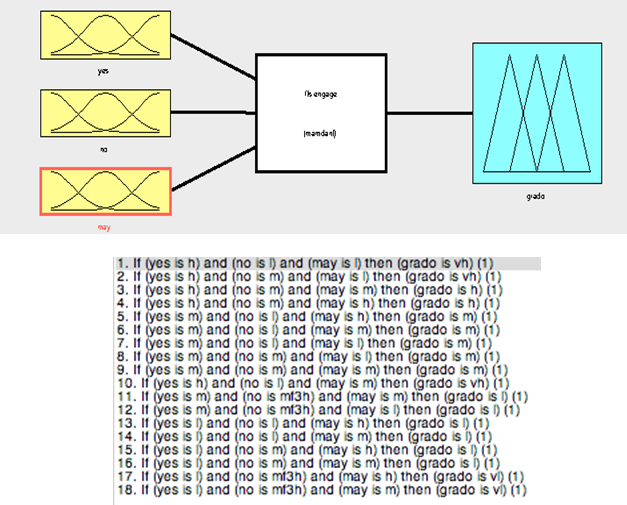
\includegraphics[scale=0.5]{fuzzyengs}
\quad  
\caption{Fuzzy Classifier Setup.}  
\label{fuzz}  
\end{figure}

%Los resultados de clasificacion fueron bastante bajos dando un 59\% de presicion como lo podemos observar en la figura \ref{fuzzyeng} se le realizaron ajustes al clasificador pero no superamos ese porcentaje por lo que optamos por usar otros clasificadores. Acontinuacion se muestran los resultados obtenidos con diferentes clasificadores.
The results of classification were quite low giving a 59 \% of pressure as we can see in the figure \ref{fuzzyeng} adjustments were made to the classifier but we did not exceed that percentage so we chose to use other classifiers. The results obtained with different classifiers are shown below.

\begin{figure}[ht!]  
\centering  
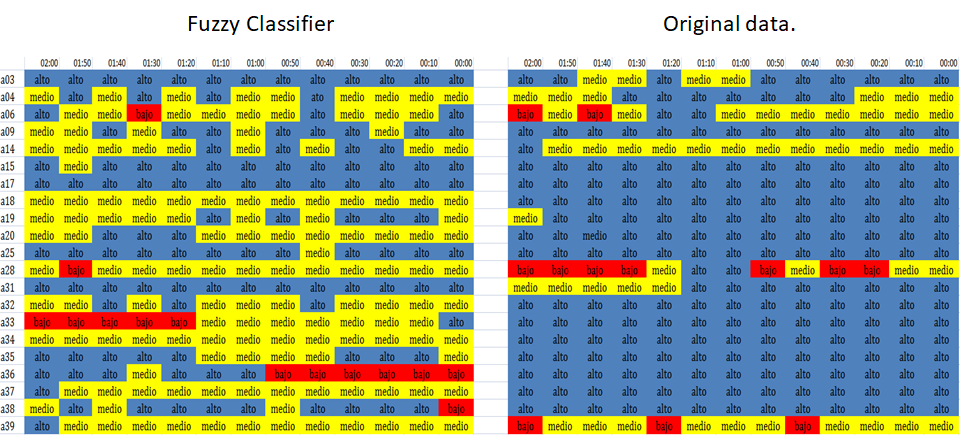
\includegraphics[scale=.5]{fuzzyeng}
\quad  
\caption{Fuzzy Classifier results vs Original Classifier.}  
\label{fuzzyeng}  
\end{figure}

\begin{table}
\small
\centering
\captionsetup{font=footnotesize}
\caption{Desicion tree}
\label{tab:detree} 
\small
\begin{tabular}{p{2cm} p{2cm} p{2cm} p{2cm} p{3cm} }
\hline{\smallskip}
 &	true Low	&	true Mid	&	true High	&	class precision\\	
\noalign{\smallskip}\hline\noalign{\smallskip}
\small{	pred. Low	}& \small{	141	}& \small{	25	}& \small{	2	}& \small{	83.93\%	}\\
\small{	pred. Mid	}& \small{	14	}& \small{	77	}& \small{	16	}& \small{	71.96\%	}\\
\small{	pred. High	}& \small{	3	}& \small{	11	}& \small{	325	}& \small{	95.87\%	}\\
\small{	class recall	}& \small{	89.24\%	}& \small{	68.14\%	}& \small{	94.75\%	}& \small{		}\\
\hline
\end{tabular}
\begin{tabular}{p{5cm} p{5cm}  }
\small{	accuracy: 88.42\% +/- 5.17\% (mikro: 88.44\%)	}& \small{	kappa: 0.803 +/- 0.088 (mikro: 0.804)	}\\
\end{tabular}
\end{table}

\begin{table}
\small
\centering
\captionsetup{font=footnotesize}
\caption{KNN}
\label{tab:Knn} 
\small
\begin{tabular}{p{2cm} p{2cm} p{2cm} p{2cm} p{3cm} }
\hline{\smallskip}
 &	true Low	&	true Mid	&	true High	&	class precision\\	
\noalign{\smallskip}\hline\noalign{\smallskip}
\small{	pred. Low	}& \small{	133	}& \small{	19	}& \small{	3	}& \small{	85.81\%	}\\
\small{	pred. Mid	}& \small{	22	}& \small{	78	}& \small{	12	}& \small{	69.64\%	}\\
\small{	pred. High	}& \small{	3	}& \small{	16	}& \small{	328	}& \small{	94.52\%	}\\
\small{	class recall	}& \small{	84.18\%	}& \small{	69.03\%	}& \small{	95.63\%	}& \small{		}\\
\hline
\end{tabular}
\begin{tabular}{p{5cm} p{5cm}  }
\small{	accuracy: 87.77\% +/- 4.13\% (mikro: 87.79\%)							}& \small{	kappa: 0.792 +/- 0.069 (mikro: 0.791)	}\\

\end{tabular}
\end{table}
\begin{table}
\small
\centering
\captionsetup{font=footnotesize}
\caption{Bayes}
\label{tab:Bays} 
\small
\begin{tabular}{p{2cm} p{2cm} p{2cm} p{2cm} p{3cm} }
\hline{\smallskip}
 &	true Low	&	true Mid	&	true High	&	class precision\\	
\noalign{\smallskip}\hline\noalign{\smallskip}
\small{	pred. Low	}& \small{	123	}& \small{	13	}& \small{	2	}& \small{	89.13\%	}\\
\small{	pred. Mid	}& \small{	13	}& \small{	64	}& \small{	14	}& \small{	70.33\%	}\\
\small{	pred. High	}& \small{	22	}& \small{	36	}& \small{	327	}& \small{	84.94\%	}\\
\small{	class recall	}& \small{	77.85\%	}& \small{	56.64\%	}& \small{	95.34\%	}& \small{		}\\
\hline
\end{tabular}
\begin{tabular}{p{5cm} p{5cm}  }
\small{	accuracy: 83.69\% +/- 4.57\% (mikro: 83.71\%)							}& \small{	kappa: 0.712 +/- 0.079 (mikro: 0.712)	}\\
\end{tabular}
\end{table}


\begin{table}
\small
\centering
\captionsetup{font=footnotesize}
\caption{Neural Network}
\label{tab:NN} 
\small
\begin{tabular}{p{2cm} p{2cm} p{2cm} p{2cm} p{3cm} }
\hline{\smallskip}
 &	true Low	&	true Mid	&	true High	&	class precision\\	
\noalign{\smallskip}\hline\noalign{\smallskip}
\small{	pred. Low	}& \small{	144	}& \small{	11	}& \small{	3	}& \small{	91.14\%	}\\
\small{	pred. Mid	}& \small{	12	}& \small{	88	}& \small{	13	}& \small{	77.88\%	}\\
\small{	pred. High	}& \small{	2	}& \small{	14	}& \small{	327	}& \small{	95.34\%	}\\
\small{	class recall	}& \small{	91.14\%	}& \small{	77.88\%	}& \small{	95.34\%	}& \small{		}\\
\hline
\end{tabular}
\begin{tabular}{p{5cm} p{5cm}  }
\small{	accuracy: 91.03\% +/- 3.68\% (mikro: 91.04\%)									}\\

\end{tabular}
\end{table}

\begin{table}
\small
\centering
\captionsetup{font=footnotesize}
\caption{SVM High and Low}
\label{tab:SVMhl} 
\small
\begin{tabular}{p{2cm} p{2cm} p{2cm} p{3cm} }
\hline{\smallskip}
 &	true High	&	true Low	&	class precision\\	
\noalign{\smallskip}\hline\noalign{\smallskip}
\small{	pred. High	}& \small{	331	}& \small{	29	}& \small{	91.94\%	}\\
\small{	pred. Low	}& \small{	12	}& \small{	129	}& \small{	91.49\%	}\\
\small{	class recall	}& \small{	96.50\%	}& \small{	81.65\%	}& \small{		}\\
\hline
\end{tabular}
\begin{tabular}{p{5cm} p{5cm}  }
\small{	accuracy: 91.82\% +/- 3.27\% (mikro: 92.11\%)}\\

\end{tabular}
\end{table}

\begin{table}
\small
\centering
\captionsetup{font=footnotesize}
\caption{SVM High and Low}
\label{tab:SVMhm} 
\small
\begin{tabular}{p{2cm} p{2cm} p{2cm} p{3cm} }
\hline{\smallskip}
 &	true High	&	true Mid	&	class precision\\	
\noalign{\smallskip}\hline\noalign{\smallskip}
\small{	pred. High	}& \small{	336	}& \small{	29	}& \small{	92.05\%	}\\
\small{	pred. Mid	}& \small{	7	}& \small{	84	}& \small{	92.31\%	}\\
\small{	class recall	}& \small{	97.96\%	}& \small{	74.34\%	}& \small{		}\\

\hline
\end{tabular}
\begin{tabular}{p{5cm} p{5cm}  }
\small{	accuracy: 92.11\% +/- 3.27\% (mikro: 92.11\%)}\\

\end{tabular}
\end{table}
\begin{table}
\small
\centering
\captionsetup{font=footnotesize}
\caption{SVM Mid and Low}
\label{tab:SVMhm} 
\small
\begin{tabular}{p{2cm} p{2cm} p{2cm} p{3cm} }
\hline{\smallskip}
 &	true Mid	&	true Low	&	class precision\\	
\noalign{\smallskip}\hline\noalign{\smallskip}
\small{	pred. Low	}& \small{	149	}& \small{	31	}& \small{	82.78\%	}\\
\small{	pred. Mid	}& \small{	8	}& \small{	82	}& \small{	91.11\%	}\\
\small{	class recall	}& \small{	94.90\%	}& \small{	72.57\%	}& \small{		}\\
\hline
\end{tabular}
\begin{tabular}{p{5cm} p{5cm}  }
\small{	accuracy: 85.56\% +/- 3.27\% (mikro: 85.56\%)}\\

\end{tabular}
\end{table}

\begin{table}
\small
\centering
\captionsetup{font=footnotesize}
\caption{Results of all the classifiers used.}
\label{tab:Allclass} 
\small
\begin{tabular}{p{3cm} p{1cm} p{1cm} p{1cm} p{2cm} }
\hline{\smallskip}
Classifier & Accuracy\\
\noalign{\smallskip}\hline\noalign{\smallskip}
\small{	Decision Tree	}& \small{	88.42\% +/- 5.17\%	}\\
\small{	KNN	}& \small{	87.77\% +/- 4.13\%	}\\
\small{	Bayes	}& \small{	83.69\% +/- 4.57\%	}\\
\small{	Neural Network	}& \small{	91.03\% +/- 3.68\% 	}\\
\small{	SVM1	}& \small{	89.83\%	}\\
\hline
\end{tabular}
\end{table}
%Todos los clasificadores se configuraron basicamente y ninguno esta optimizado por lo que todos los resultados se pueden mejorar ahora el clasificador que mejor resultado tubo fue la red neuronal con un 91.03\% de presicion en cuanto a la clasificacion de el nivel de atencion de los usuarios, para reforsar estos resultados adicionalmente encuestamos a los usuarios para tener una idea si los gustos de los usuarios son consistentes con su nivel de atencion en la tabla X podemos observar estos datos. 
All classifiers were configured basically and none is optimized so that all the results can be improved now the classifier that best result tube was the neural network with a 91.03\% of pressure in terms of the classification of the level of attention of users , To reinforce these results additionally we survey the users to get an idea if the tastes of the users are consistent with their level of attention in table \ref{tab:surv3} we can observe this data.
\begin{landscape}
\begin{table}
\small
\centering
\captionsetup{font=footnotesize}
\caption{Sample of data provided by the video footage.}
\label{tab:surv3} 
\small
\begin{tabular}{p{0.5cm} p{0.5cm} p{0.5cm} p{0.5cm} p{0.5cm}p{0.5cm} p{0.5cm} p{0.5cm} p{0.5cm} p{0.5cm}p{0.5cm} p{0.5cm} p{0.5cm} p{0.5cm} p{0.5cm}p{0.5cm} p{2cm} p{0.5cm} }
\hline{\smallskip}
User	&	1	&	2	&	3	&	4	&	5	&	6	&	7	&	8	&	9	&	10	&	11	&	12	&	13	&	14	&	15	&	Gender	&	Age	\\
\noalign{\smallskip}\hline\noalign{\smallskip}
\small{	a0	}& \small{	5	}& \small{	4	}& \small{	2	}& \small{	1	}& \small{	5	}& \small{	1	}& \small{	2	}& \small{	2	}& \small{	1	}& \small{	1	}& \small{	5	}& \small{	2	}& \small{	2	}& \small{	3	}& \small{	4	}& \small{			Male 	}& \small{	19	}\\
\small{	a1	}& \small{	4	}& \small{	5	}& \small{	3	}& \small{	5	}& \small{	5	}& \small{	4	}& \small{	2	}& \small{	1	}& \small{	5	}& \small{	5	}& \small{	5	}& \small{	4	}& \small{	4	}& \small{	3	}& \small{	4	}& \small{			Male	}& \small{	19	}\\
\small{	a2	}& \small{	3	}& \small{	4	}& \small{	3	}& \small{	5	}& \small{	5	}& \small{	5	}& \small{	4	}& \small{	3	}& \small{	4	}& \small{	2	}& \small{	4	}& \small{	5	}& \small{	5	}& \small{	3	}& \small{	5	}& \small{			Male	}& \small{	21	}\\
\small{	a3	}& \small{	3	}& \small{	2	}& \small{	2	}& \small{	4	}& \small{	5	}& \small{	2	}& \small{	3	}& \small{	4	}& \small{	5	}& \small{	3	}& \small{	2	}& \small{	5	}& \small{	4	}& \small{	4	}& \small{	5	}& \small{			Female	}& \small{	20	}\\
\small{	a4	}& \small{	5	}& \small{	5	}& \small{	5	}& \small{	5	}& \small{	5	}& \small{	5	}& \small{	5	}& \small{	3	}& \small{	4	}& \small{	4	}& \small{	5	}& \small{	5	}& \small{	4	}& \small{	1	}& \small{	5	}& \small{			Male	}& \small{	25	}\\
\small{	a5	}& \small{	5	}& \small{	5	}& \small{	3	}& \small{	5	}& \small{	5	}& \small{	2	}& \small{	5	}& \small{	4	}& \small{	3	}& \small{	3	}& \small{	5	}& \small{	4	}& \small{	5	}& \small{	5	}& \small{	5	}& \small{			Male	}& \small{	19	}\\
\small{	a6	}& \small{	3	}& \small{	3	}& \small{	2	}& \small{	4	}& \small{	3	}& \small{	3	}& \small{	3	}& \small{	1	}& \small{	4	}& \small{	2	}& \small{	4	}& \small{	3	}& \small{	3	}& \small{	4	}& \small{	4	}& \small{			Female	}& \small{	20	}\\
\small{	a7	}& \small{	2	}& \small{	4	}& \small{	4	}& \small{	5	}& \small{	5	}& \small{	3	}& \small{	1	}& \small{	4	}& \small{	5	}& \small{	3	}& \small{	4	}& \small{	4	}& \small{	1	}& \small{	2	}& \small{	3	}& \small{			Male	}& \small{	22	}\\
\small{	a8	}& \small{	1	}& \small{	3	}& \small{	3	}& \small{	5	}& \small{	5	}& \small{	4	}& \small{	5	}& \small{	5	}& \small{	4	}& \small{	1	}& \small{	5	}& \small{	1	}& \small{	4	}& \small{	5	}& \small{	3	}& \small{			Male 	}& \small{	25	}\\
\small{	a9	}& \small{	5	}& \small{	5	}& \small{	3	}& \small{	3	}& \small{	4	}& \small{	3	}& \small{	2	}& \small{	4	}& \small{	5	}& \small{	1	}& \small{	3	}& \small{	5	}& \small{	5	}& \small{	1	}& \small{	4	}& \small{			Male 	}& \small{	21	}\\
\small{	a10	}& \small{	4	}& \small{	4	}& \small{	4	}& \small{	5	}& \small{	4	}& \small{	5	}& \small{	3	}& \small{	2	}& \small{	2	}& \small{	2	}& \small{	4	}& \small{	5	}& \small{	4	}& \small{	4	}& \small{	5	}& \small{			Male 	}& \small{	25	}\\
\small{	...	}& \small{	...	}& \small{	...	}& \small{	...	}& \small{	...	}& \small{	...	}& \small{	...	}& \small{	...	}& \small{	...	}& \small{	...	}& \small{	...	}& \small{	...	}& \small{	...	}& \small{	...	}& \small{	...	}& \small{	...	}& \small{			... 	}& \small{	...	}\\
\small{	a35	}& \small{	5	}& \small{	5	}& \small{	5	}& \small{	5	}& \small{	5	}& \small{	5	}& \small{	4	}& \small{	4	}& \small{	5	}& \small{	1	}& \small{	5	}& \small{	5	}& \small{	1	}& \small{	4	}& \small{	5	}& \small{			Female	}& \small{	25	}\\
\small{	a36	}& \small{	4	}& \small{	5	}& \small{	4	}& \small{	4	}& \small{	4	}& \small{	3	}& \small{	3	}& \small{	2	}& \small{	3	}& \small{	4	}& \small{	5	}& \small{	5	}& \small{	3	}& \small{	5	}& \small{	5	}& \small{			Female	}& \small{	22	}\\
\small{	a37	}& \small{	4	}& \small{	4	}& \small{	4	}& \small{	5	}& \small{	4	}& \small{	4	}& \small{	4	}& \small{	3	}& \small{	3	}& \small{	2	}& \small{	4	}& \small{	5	}& \small{	3	}& \small{	3	}& \small{	4	}& \small{			Male 	}& \small{	22	}\\
\small{	a38	}& \small{	2	}& \small{	2	}& \small{	1	}& \small{	4	}& \small{	3	}& \small{	2	}& \small{	2	}& \small{	2	}& \small{	1	}& \small{	5	}& \small{	1	}& \small{	1	}& \small{	1	}& \small{	2	}& \small{	3	}& \small{			Female	}& \small{	32	}\\
\small{	a39	}& \small{	4	}& \small{	5	}& \small{	3	}& \small{	5	}& \small{	5	}& \small{	3	}& \small{	5	}& \small{	3	}& \small{	2	}& \small{	2	}& \small{	5	}& \small{	3	}& \small{	5	}& \small{	4	}& \small{	5	}& \small{			Male 	}& \small{	30	}\\
\small{	a40	}& \small{	4	}& \small{	4	}& \small{	1	}& \small{	3	}& \small{	3	}& \small{	1	}& \small{	2	}& \small{	2	}& \small{	3	}& \small{	5	}& \small{	2	}& \small{	5	}& \small{	4	}& \small{	1	}& \small{	4	}& \small{			Male	}& \small{	38	}\\

\hline
\end{tabular}
\end{table}
\end{landscape}